\documentclass[draft]{homework}

\usepackage{graphicx}
\usepackage{xspace}


\newcommand{\kat}{Kathará\xspace}
\newcommand{\opn}{OPNsense\xspace}
\newcommand{\vb}{VirtualBox\xspace}

\newcommand{\client}{\textit{client}\xspace}
\newcommand{\dmz}{\textit{DMZ}\xspace}
\newcommand{\ser}{\textit{internal server}\xspace}
\newcommand{\intfw}{\textit{intfw}\xspace}
\newcommand{\mainfw}{\textit{mainfw}\xspace}

\newcommand{\lan}{\textit{LAN}\xspace}
\newcommand{\opt}{\textit{OPT1}\xspace}
\newcommand{\wan}{\textit{WAN}\xspace}


\title{Practical Network Defense - Lab 6}
\author{Alessandro Serpi - 1647244}
\date{3 May 2019}


\begin{document}
    \maketitle
    \tableofcontents
    
    
    \pagebreak
    \section{Introduction}
    \fxnote{TODO}
    
    
    \section{Zentyal configuration}
    \fxnote{TODO}
    
    
    \section{\opn internal firewall configuration}
    \subsection{Server}
    Create a new authentication server in \textit{System} $\rightarrow$ \textit{Access} $\rightarrow$ \textit{Server} with the following settings:
    \begin{figure}[H]
        \centering
        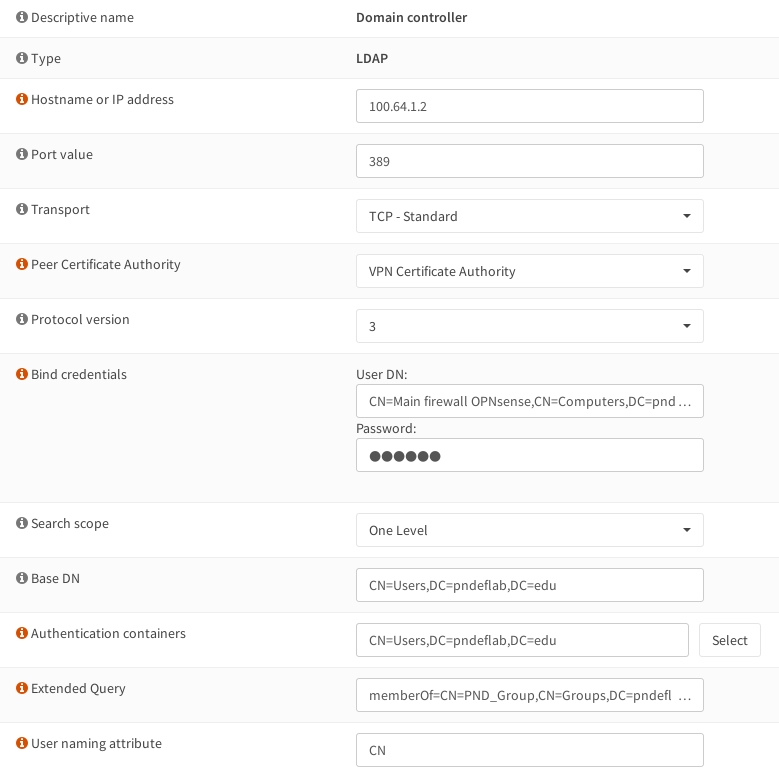
\includegraphics[width=\linewidth]{images/server}
        \label{fig:server}
    \end{figure}
    In field \textit{Bind credential}, insert the distinguished name and password for the \intfw account created in the domain controller.
    In field \textit{Extended query}, specify that the users must be member of the \textit{PND\_Group} group.
    After completing the form up to \textit{Base DN}, press the \textit{Select} button adjacent to field \textit{Authentication containers} and choose the only option available.
    
    \subsection{Users}
    In \textit{System} $\rightarrow$ \textit{Access} $\rightarrow$ \textit{Users}, import start importing new users clicking on the cloud icon.
    Select all showed users and insert them in the \textit{admin} group.
    
    \subsection{Settings}
    In \textit{System} $\rightarrow$ \textit{Settings} $\rightarrow$ \textit{Administration}, change the authentication server to \textit{Domain controller}.
    Since superuser access is disabled, it may be advisable to add \textit{admin} to the list of sudoers.
    \begin{figure}[H]
        \centering
        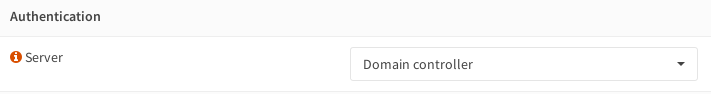
\includegraphics[width=\linewidth]{images/settings}
        \label{fig:settings}
    \end{figure}
    
    If SSH is enabled, add \textit{admin} to the SSH login groups and disable root login.
    
    
    \section{\opn main firewall configuration}
    Follow the configuration section for the internal firewall, changing the bind account to the one created for \textit{mainfw}.
    In the internal firewall, create a rule for allowing LDAP traffic from the main firewall to the domain controller.
    \begin{figure}[H]
        \centering
        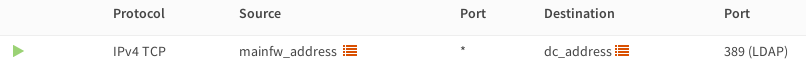
\includegraphics[width=\linewidth]{images/rule}
        \label{fig:rule}
    \end{figure}
    
    
    \section{Test of the configuration}
    Testing was performed manually, trying to login in the two firewalls, both in the web GUI and the physical terminal.
    Using the built-in root user had a negative outcome, while using a LDAP account gave access to both the web GUI and the shell.
    
    
    \section{Final remarks}
    \opn has a lacklustre LDAP support.
    
    The primary shortcoming is the manual user configuration: the usefulness of a central domain controller is greatly diminished if admins must import locally and configure new users in each firewall.
    
    Another deficiency is the non-existent group support.
    A sensible approach would be inserting newly-imported users into local groups with the same names as their LDAP groups (optionally creating those which do not exist) in order to ease privilege assignment; instead, LDAP groups are completely ignored.
    
    Lastly, the documentation is not up to date: some icons are different (e.g. the user import icon) and some settings are located in different sections (e.g. the active authentication servers).
\end{document}
